%!TEX root = ../risk_book.tex

\chapter{A comparison of economics, health, and political risks}


Key participants were first tallied (\texttt{/NN.?/ \textgreater \textgreater \# (NP !> PP)}) in order to broadly understand the key social actors in the three subcorpora (see Figure \ref{fig:clouds}).

			\begin{figure}[htb!]
			\centering
			\addvbuffer[12pt 8pt]{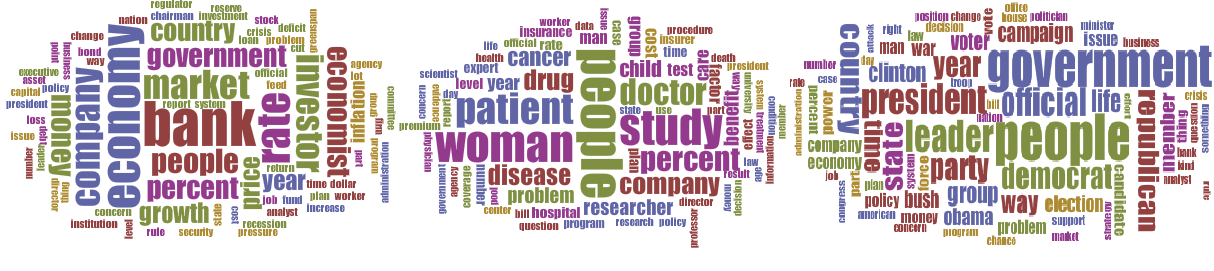
\includegraphics[width=0.75\textwidth]{../images/clouds.png}}
			\caption{Key participants in the \emph{Economics}, \emph{Health} and \emph{Politics} subcorpora}
			\label{fig:clouds}
			\end{figure}

			\begin{figure}[htb!]
			\centering
			\addvbuffer[12pt 8pt]{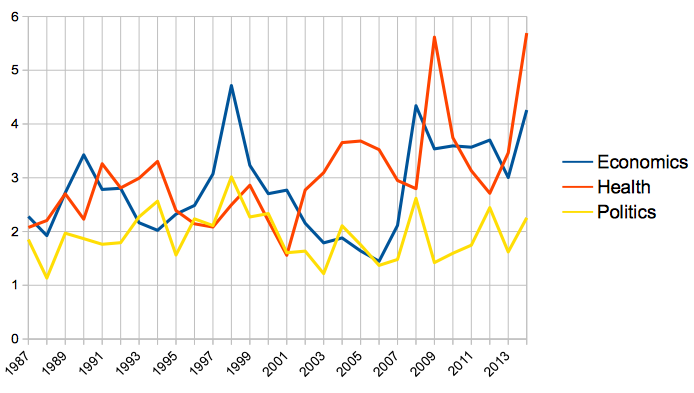
\includegraphics[width=.70\textwidth]{../images/echepol_riskwords.png}}
			\caption{Risk words per total number of article topics per year}
			\label{fig:echepol_riskwords}
			\end{figure}
			%
			Due to time constraints, we restricted the topic comparison to domains that had yielded interesting insights in the earlier interrogations. Further, we found that the smaller size of the subcorpora limited us to lexicogrammatical queries that outputted a large enough number of results for quantitative reliablity. Thus, we focussed on the following three areas:

		 	\begin{table}[htb!]
		 	\centering
		 	\small
		 	\begin{tabular}{|l|l|l|}
		 			 	\hline
		 			 	\textbf{Economics}   & \textbf{Health}         & \textbf{Politics}     \\ \hline
		 			 	political   & high           & political    \\ \hline
		 			 	big         & great          & great        \\ \hline
		 			 	economic    & low            & big          \\ \hline
		 			 	financial   & other          & high         \\ \hline
		 			 	great       & serious        & own          \\ \hline
		 			 	high        & financial      & serious      \\ \hline
		 			 	more        & potential      & new          \\ \hline
		 			 	real        & medical        & real         \\ \hline
		 			 	systemic    & more           & considerable \\ \hline
		 			 	significant & significant    & more         \\ \hline
		 			 	new         & cardiovascular & other        \\ \hline
		 			 	little      & political      & significant  \\ \hline
		 			 	global      & possible       & economic     \\ \hline
		 			 	serious     & small          & financial    \\ \hline
		 			 	other       & real           & potential    \\ \hline
		 			 	excessive   & such           & personal     \\ \hline
		 			 	potential   & genetic        & little       \\ \hline
		 			 	such        & ovarian        & such         \\ \hline
		 			 	much        & same           & public       \\ \hline
		 			 	own         & bad            & military     \\ \hline
		 			 	\end{tabular}
		 			 	\caption{Most common adjectives modifying nominal risks in the topic subcorpora}
		 			 	\label{tab:echepo_adjmod}
		 	\end{table}

\section{Summary}

	Unlike the general corpus of all articles, these subcorpora made it possible to observe the influence of key events:

	\begin{enumerate}
		\item Event 1 and 2 in Economics
		\item Event 1 and 2 in Health
		\item Event 1 and 2 in subcorpus 3
	\end{enumerate}





%\bibliography{../references/libwin}